\chapter{Creeping flow}
\label{ch:creepflow}

\section{Learning objectives}

At the end of this lesson, a student should be able to

\begin{enumerate}
\item list the assumptions and concepts behind Stoke's law
\item recollect the Stoke's law
\item apply Stoke's law to simple problems of force balance
\end{enumerate}


\section{Concept map}

A concept map exposing the connection between different concepts behind Stoke's law is given in the figure~\ref{StokesConceptMap}.

\index{Concept map, Stokes law}
\begin{figure}[h]
\begin{center}
\resizebox{!}{4in}{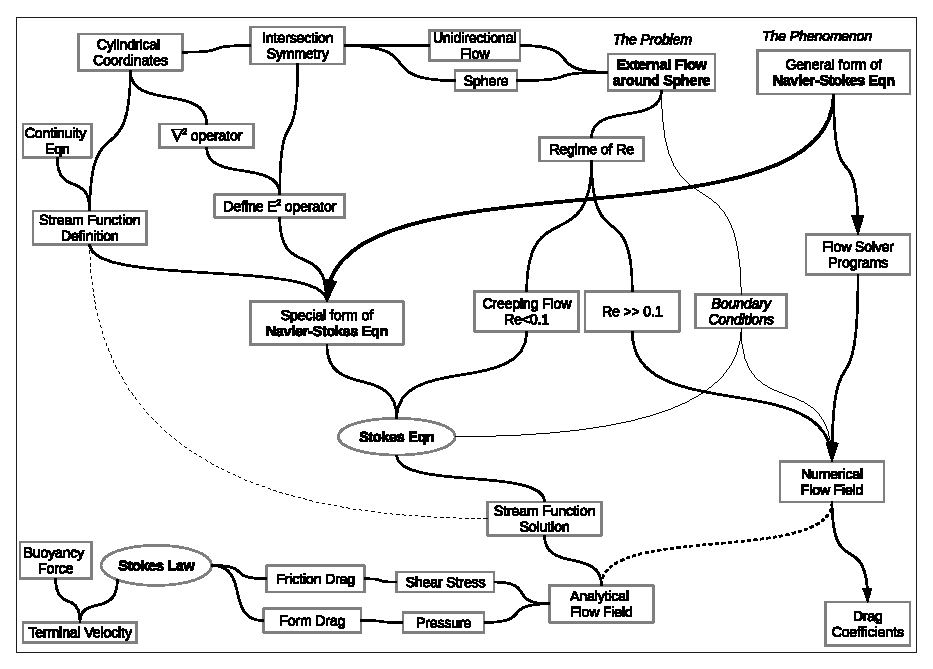
\includegraphics{images/c13-StokesLawConceptMap.eps}}
\end{center}
\caption{Concept map for Stokes law derivation}
\label{StokesConceptMap}
\end{figure}

\section{N-S equations using stream function}

The Navier-Stokes equations can be written for 2D flow without body force term as follows:

\begin{equation}
\label{nsa2D1}
\frac{\partial u_1}{\partial t} + u_1\frac{\partial u_1}{\partial x_1} + u_2\frac{\partial u_1}{\partial x_2} = -  \frac{1}{\rho}\frac{\partial p}{\partial x_1} + \nu \left( \frac{\partial^2 u_1}{\partial x_1^2} + \frac{\partial^2 u_1}{\partial x_2^2} \right)
\end{equation} 

\begin{equation}
\label{nsa2D2}
\frac{\partial u_2}{\partial t} + u_1\frac{\partial u_2}{\partial x_1} + u_2\frac{\partial u_2}{\partial x_2} = -  \frac{1}{\rho}\frac{\partial p}{\partial x_2} + \nu \left( \frac{\partial^2 u_2}{\partial x_1^2} + \frac{\partial^2 u_2}{\partial x_2^2} \right)
\end{equation} 

Differentiate eqn~\ref{nsa2D1} with respect to $x_2$ and eqn~\ref{nsa2D2} with respect to $x_1$ and substract the second from the first.

\begin{eqnarray}
\label{nsa2Ds}
\frac{\partial }{\partial t} \left( \frac{\partial u_1}{\partial x_2} - \frac{\partial u_2}{\partial x_1} \right) + \\ \nonumber
\frac{\partial}{\partial x_2} \left[ u_1\frac{\partial u_2}{\partial x_1} + u_2\frac{\partial u_2}{\partial x_2} \right] -  & \\ \nonumber
\frac{\partial}{\partial x_1} \left[u_1\frac{\partial u_2}{\partial x_1} + u_2\frac{\partial u_2}{\partial x_2} \right] 
  = & \nu \frac{\partial}{\partial x_2} \left[ \frac{\partial^2 u_2}{\partial x_1^2} + \frac{\partial^2 u_2}{\partial x_2^2} \right] - \\ \nonumber
 & \nu \frac{\partial}{\partial x_1} \left[ \frac{\partial^2 u_2}{\partial x_1^2} + \frac{\partial^2 u_2}{\partial x_2^2} \right]
\end{eqnarray}

From the definition of $u_1$ and $u_2$ using a stream function $\psi$, it is easy to note the following simplification.

\begin{equation}
\label{nsa2Ds1}
\frac{\partial u_1}{\partial x_2} - \frac{\partial u_2}{\partial x_1} = \nabla^2 \psi
\end{equation}



One can simplify the R.H.S. of eqn~\ref{nsa2Ds} to the following:

Define a new operator $\nabla^4$ as follows:

$$ \nabla^4 \psi \equiv \nabla^2 \nabla^2 \psi$$

\begin{equation} 
\label{nsa2Ds2}
\frac{\partial}{\partial x_2} \left[ \frac{\partial^2 u_2}{\partial x_1^2} + \frac{\partial^2 u_2}{\partial x_2^2} \right] - \frac{\partial}{\partial x_1} \left[ \frac{\partial^2 u_2}{\partial x_1^2} + \frac{\partial^2 u_2}{\partial x_2^2} \right] = \nabla^4 \psi
\end{equation} 

$$ {\partial \nabla^2 \psi \over \partial t} + \left[ {\partial \over \partial x_2} \left( \vec{u}\cdot \vec{\nabla} u_1 \right) - {\partial \over \partial x_1}\left( \vec{u}\cdot \vec{\nabla} u_2 \right) 	\right] = \nu \nabla^4 \psi $$ 


Expanding the velocities using the stream function, the term in the square brackets can be simplified to be the following.
{\bf any error here?}

$$\left[ {\partial \over \partial x_2} \left( \vec{u}\cdot \vec{\nabla} u_1 \right) - {\partial  \over \partial x_1}\left( \vec{u}\cdot \vec{\nabla} u_2 \right)	\right] = {\partial \psi \over \partial x_2} {\partial \over \partial x_1} \nabla^2 \psi - {\partial \psi \over \partial x_1} {\partial \over \partial x_2} \nabla^2 \psi $$

\begin{quote}
{\bf Classwork:} Convince yourself about the above expression by substituting for the velocity components and using differentiation by parts.
\end{quote}

\begin{equation}
\frac{\partial}{\partial x_2} \left[ u_1\frac{\partial u_2}{\partial x_1} + u_2\frac{\partial u_2}{\partial x_2} \right] - \frac{\partial}{\partial x_1} \left[u_1\frac{\partial u_2}{\partial x_1} + u_2\frac{\partial u_2}{\partial x_2} \right] = - \left[ \frac{\partial \psi}{\partial x_1} \frac{\partial \nabla^2 \psi}{\partial x_2} - \frac{\partial \psi}{\partial x_2} \frac{\partial \nabla^2 \psi}{\partial x_1} \right]
\end{equation}


We now define the following expression using the Jacobian notation of determinant of a matrix as follows.

\begin{equation*}
 {\partial \left( \psi, \nabla^2 \psi \right) \over \partial \left( x_1, x_2 \right) } \equiv
\begin{vmatrix}
{\partial \psi \over \partial x_1} & {\partial \psi \over \partial x_2} \\
\ \\
{\partial \over \partial x_1} \nabla^2 \psi & {\partial \over \partial x_2} \nabla^2 \psi \\
\end{vmatrix}
\end{equation*}


The R.H.S. of the above equation can be written as Jacobian Determinant in 2D as follows.

\begin{equation}
\label{nsa2Ds3}
\left[ \frac{\partial \psi}{\partial x_1} \frac{\partial \nabla^2 \psi}{\partial x_2} - \frac{\partial \psi}{\partial x_2} \frac{\partial \nabla^2 \psi}{\partial x_1} \right] = \frac{\partial \left( \psi, \nabla^2 \psi\right)}{\partial\left(x_1, x_2\right)}
\end{equation}

Combining equations ~\ref{nsa2Ds1}, ~\ref{nsa2Ds1} and \ref{nsa2Ds3} with \ref{nsa2Ds}, we get the Navier-Stokes equation in 2D, without body force term using stream function $\psi$ as follows:

\begin{equation}
\label{nsa2Ds4}
\boxed{
\frac{\partial \nabla^2 \psi}{\partial t} -  \frac{\partial \left( \psi, \nabla^2 \psi\right)}{\partial\left(x_1, x_2\right)} = \nu \nabla^4 \psi
}
\end{equation}


\section{The $E^2$ operator}

As can be seen above, the Laplacian operator is an important operator for the stream function use. The definition of this operator for different coordinate systems is as follows.


Laplacian in rectangular coordinates:

$$ \nabla^2 \equiv {\partial^2 \over \partial x^2} + {\partial^2 \over \partial y^2} + {\partial^2 \over \partial z^2} $$


Laplacian in cylindrical coordinates:

$$ \nabla^2 \equiv {1 \over r} {\partial \over \partial r} \left( r {\partial \over \partial r} \right) + {1 \over r^2} {\partial^2 \over \partial \theta^2} + {\partial^2 \over \partial z^2} $$


Laplacian in spherical coordinates:

$$ \nabla^2 \equiv {1 \over r^2} {\partial \over \partial r} \left( r^2 {\partial \over \partial r} \right) + {1 \over r^2 \sin\theta} {\partial \over \partial \theta} \left( \sin \theta {\partial \over \partial \theta } \right) + {1 \over r^2 \sin^2\theta} {\partial^2 \over \partial \phi^2} $$

The Laplacian operator and the Navier-Stokes equation take special forms for 2D flow in cylindrical and spherical coordinates if additional symmetry is imposed on the flow field.


{\bf Cylindrical with $V_z=0$ and no $z$ dependence:}

$$ \nabla^2 = {\partial^2 \over \partial r^2} + {1 \over r} {\partial \over \partial r} + {1 \over r^2} {\partial^2 \over \partial \theta^2} $$

Navier-Stokes equation for this situation reduces to:

$$ {\partial \over \partial t} \left( \nabla^2 \psi \right) - {1 \over r} {\partial\left( \psi, \nabla^2 \psi\right) \over \left(r, \theta \right)} = \nu \nabla^4 \psi $$


In situations where the flow is axisymmetrical, we need to define a new operator $E$ as follows:


{\bf Cylindrical with $V_\theta=0$ and no $\theta$ dependence:}

$$ E^2 \equiv {\partial^2 \over \partial r^2} - {1 \over r} {\partial \over \partial r} + {\partial^2 \over \partial z^2} $$

Navier-Stokes equation for this situation reduces to:

$$ {\partial \over \partial t} \left( E^2 \psi \right) - {1 \over r} {\partial\left( \psi, E^2 \psi\right) \over \left(r, z \right)} - {2 \over r^2} {\partial \psi \over \partial z} E^2 \psi = \nu E^4 \psi $$


Note the difference in the operator used and the reduced form of Navier-Stokes equation in the above two situations for a 2D flow in cylindrical coordinate system. 

{\bf Spherical with $V_\phi =0$ and no $\phi$ dependence:}


$$ E^2 \equiv {\partial^2 \over \partial r^2} + {\sin \theta \over r^2} {\partial \over \partial \theta} \left( {1 \over \sin\theta} {\partial \over \partial \theta} \right) $$

Navier-Stokes equation in this situation reduces to:

$$ {\partial \over \partial t} \left( E^2 \psi \right) - {1 \over r^2 \sin\theta} {\partial\left( \psi, E^2 \psi\right) \over \left(r, \theta \right)} + {2 E^2 \psi \over r^2 \sin^2\theta} \left( {\partial \psi \over \partial r} \cos\theta - {1 \over r} {\partial \psi \over \partial \theta} \sin\theta \right) = \nu E^4 \psi $$


In both the above situations, the $E^4$ is defined as $E^2 \left(E^2 \right)$.


Note the difference in the definition of $E^2$ for the cylindrical and spherical coordinates.


\section{Creeping flow over a sphere}

\index{Creeping flow}

When $Re < 0.1$, the flow around a smooth sphere is such that the viscous
effects are present all around the sphere and no \textit{flow separation} takes
place. For such a flow regime called \textit{creeping flow}. around a sphere, we
are interested not in the flow distribution around it but the viscous drag. The
velocity of a sphere falling in a liquid column (terminal velocity) or the far
field velocity of a fluid flowing around a sphere is $u_\infty$ or simply $U$ as shown in the
figure \ref{stokes}.

\begin{figure}[h]
\begin{center}
\framebox{
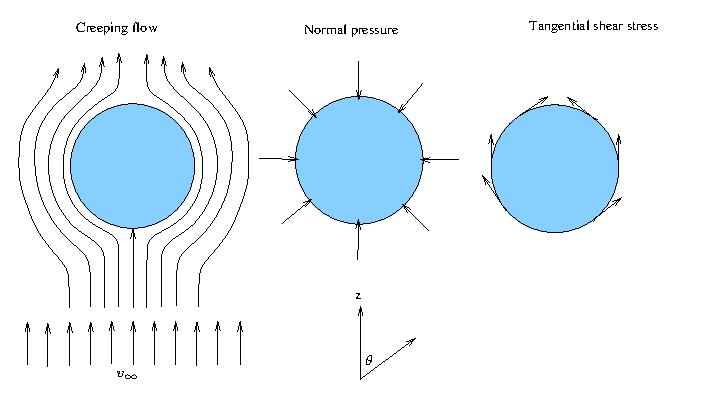
\includegraphics[scale=1.0]{images/c13-stokesfig.ps}
}
\end{center}
\caption{Creeping flow around a sphere}
\label{stokes}
\end{figure}

For very low Reynolds number, the acceleration terms can be neglected. The Navier-Stokes equation can then be approximated by the Stoke's equation. The stream-function form of Stoke's equation for this situation is given by:

$$ E^4 \psi = 0 $$

This needs to be solved for the following boundary conditions.

\begin{quote}
{\bf Classwork:} Convince yourself about the following forms of boundary conditions.
\end{quote}

$$ V_r(R,\theta) = 0 \implies {\partial \over \partial \theta} \psi(R,\theta) = 0$$

$$ V_\theta(R,\theta) = 0 \implies {\partial \over \partial r} \psi(R,\theta) = 0$$

$$ V_r(\infty,\theta) \rightarrow U \cos\theta \implies {\partial \over \partial \theta} \psi( \infty,\theta) \rightarrow  r^2 U \sin\theta \cos\theta$$

$$ V_\theta(\infty,\theta) \rightarrow -U \sin\theta \implies {\partial \over \partial r} \psi(\infty,\theta) \rightarrow rU\sin^2\theta$$

Combining the two above, we can say that the boundary condition on $\psi$ at $(\infty,\theta)$ is:

$$ \psi(\infty,\theta) \rightarrow {r^2 U \sin^2 \theta \over 2} $$

We propose that the solution of $\psi(r,\theta)$ for this problem can be of the following form.

$$ \psi(r,\theta) = f(r) \sin^2 \theta$$

We need to determine the form of $f(r)$ to satisfy the above conditions.

Substitute the proposed solution in the Stoke's equation to get the following:

$$ E^4 \psi = E^2 \left( E^2 \right) \psi = \left[ {\partial^2 \over \partial r^2} + {\sin \theta \over r^2} {\partial \over \partial \theta} \left( {1 \over \sin\theta} {\partial \over \partial \theta} \right) \right]^2 f(r) \sin^2 \theta = 0 $$


\begin{quote}
{\bf Classwork:} Convince yourself that this expression can be reduced to the following. Use differentiation by parts and simplify.
\end{quote}


$$ \left[ {\partial^2 \over \partial r^2} - {2 \over r^2} \right]^2 f(r) = 0 $$


We suspect a form of $r^n$ may satisfy this equation. 

\begin{quote}
{\bf Classwork:} Convince yourself that the above equation when used with $f(r)=r^n$ simplifies to the following. 
$$(n+1)(n-1)(n-2)(n-4)r^{n-4}=0$$.
\end{quote}


We see that the equation turns out to be true only for the values of n in $\{-1, 1, 2, 4 \}$. We take a linear combination of these four possible solutions to arrive at a general solution as follows.

$$ f(r) = A r^4 + B r^2 + Cr + {D \over r}$$

The boundary conditions for this equation shall be:

$$ f\left(R\right) = 0 $$

$$ \left. {\partial f \over \partial r} \right|_R = 0 $$

$$ f\left(\infty\right) \rightarrow {r^2 U \over 2} $$


Inspecting the boundary conditions that this expression of $f(r)$ should satisfy, we can arrive at the values of the four coefficients.

\begin{quote}
{\bf Classwork:} Show that the coefficients take the following values: \\
$A=0$, $B=U/2$, $C =-3UR/4$ and $D=UR^3/4$.
\end{quote} 

Thus, the final solution of $\psi$ comes out as follows.

$$ \psi(r,\theta) = UR^2 \sin^2 \theta \left[ {1 \over 2} \left( r \over R \right)^2 - {3 \over 4} \left(r \over R\right) + {1 \over 4} \left( R \over r\right) \right] $$

\begin{quote}
{\bf Homework:} Plot contours of the above function using, say, Matlab and convince yourself about the nature of the flow around a sphere in 2D.
\end{quote}


Using this stream function, the two velocity components can be arrived at as:

$$ V_r(r,\theta) = U \cos\theta \left[ 1 - {3 \over 2} \left( R \over r\right) + {1 \over 2} \left( R \over r\right)^3 \right] $$

$$ V_\theta(r,\theta) = - U \sin\theta \left[ 1 - {3 \over 4} \left( R \over r\right) - {1 \over 4} \left( R \over r\right)^3 \right] $$

\subsection{Pressure}

Substitute the above two velocity components in the Navier-Stokes equation, without the acceleration term as follows.

Substitute the solution for $V_r$ in the simplified form of Navier-Stokes equation for $V_r$ in spherical coordinate system:

$$ 0 = - {\partial p \over \partial r} + \mu \left[ {1 \over r^2} {\partial^2 \over \partial r^2} \left( r^2 V_r \right) + {1 \over r^2 \sin\theta}{\partial \over \partial \theta} \left( \sin \theta {\partial V_r \over \partial \theta} \right) \right] $$

This gives the first variation of pressure as follows.

$$ {\partial p \over \partial r} = {3 R \mu U } \left( 1 \over r^3 \right) \cos\theta $$

Similarly, substitute the solution for $V_\theta$ and $V_r$ in the Navier-Stokes equation for $V_\theta$ in spherical coordinate system:

$$ 0 = - {1 \over r} {\partial p \over \partial \theta} + \mu \left[ {1 \over r^2} {\partial \over \partial r} \left( r^2 {\partial V_\theta \over \partial r} \right) + {1 \over r^2}{\partial \over \partial \theta} \left( {1 \over \sin \theta} {\partial \left( V_\theta \sin\theta\right) \over \partial \theta} \right) + {2 \over r^2} {\partial V_r \over \partial \theta } \right] $$

This gives the second variation of pressure as follows.

$$ {\partial p \over \partial \theta} = {3 \over 2} {\mu U \over R} \left( R \over r \right)^2 \sin \theta $$

\begin{quote}
{\bf Classwork:} Convince yourself about the above derivatives of pressure and the below integrated form.
\end{quote}

Integrating the two, we obtain:

$$ p = - {3 \over 2} {\mu U \over R} \left( R \over r \right)^2 \cos \theta + \text{constant}$$

It turns out that the integration constant is $p_0 - \rho g z$.



\subsection{Drag forces}

We borrow the expressions for pressure and stress for creeping flow around a
sphere from section 2.6 of Bird's book on Transport Phenomena.

Pressure: 
$$p = p_0 - \rho g z - \frac{3}{2} \frac{\mu u_\infty}{R}
\left(\frac{R}{r}\right)^2 \cos\theta$$

We can choose to have $p_0 = 0$ for the following discussion.

\begin{quote}
Look up BLS book to obtain the expressions for different stresses in spherical coordinates.
\end{quote}

Shear Stress:

$$ \sigma_{rr} = \mu \left[ 2 { \partial V_r \over \partial r} \right] $$

$$ \tau_{r\theta} = \mu \left[ r {\partial \over \partial r} \left( V_\theta \over r \right) + {1 \over r} {\partial V_r \over \partial \theta} \right]$$


Substitute the expression for $V_r$ to get the following.

$$\sigma_{rr} = \frac{3\mu v_\infty}{R} \left[ -\left(\frac{R}{r}\right)^2 +
\left(\frac{R}{r}\right)^4 \right] \cos\theta$$ 


$$\tau_{r\theta} = \frac{3}{2} \frac{\mu u_\infty}{R} \left(\frac{R}{r}\right)^4
\sin\theta$$ 


An elemental area on the surface of the sphere of radius $R$ is given by $Rd\theta \, R\sin\theta d\phi = R^2 \,\sin\theta \, d\theta \, d\phi$.


Substitute $z = R \cos\theta$ in the pressure term before integrating.


\begin{quote}
{\bf Classwork:} Convince yourself about the following integration.
\end{quote}

{\bf Watch out confusion between $\theta$ and $\phi$ here. Also the integration limits correspondingly}

The normal force along $z$ due to the $z$ component of pressure and normal
stress $\tau_{rr}$ is given as:
$$ F_n = \int_{0}^{\pi}{ \int_{0}^{2\pi}{ \left( - p|_{r=R} +
\sigma_{rr}|_{r=R}\right) \cos\theta \, R^2 \sin\theta d\theta d\phi}} $$ 

$$ = \frac{4}{3} \pi R^3 \rho g + 2 \pi \mu R u_\infty $$

The first term $\frac{4}{3} \pi R^3 \rho g$ is called \textit{buoyancy force}.


The second term $2 \pi \mu R u_\infty$ is called \textit{form drag}. \index{Form drag}

\begin{quote}
{\bf Classwork:} Convince yourself about the following integration.
\end{quote}


The tangential force along $z$ due to  $z$ component of shear stress
$\tau_{r\theta}$ is given as:
$$ F_t = \int_{0}^{\pi}{ \int_{0}^{2\pi}{ \left( \tau_{r\theta}|_{r=R} \, \sin\theta \right) R^2
\sin\theta d\theta d\phi}} $$ 

$$ = 3 \pi \mu R u_\infty \int_{0}^{\pi}{\sin^3\theta d\theta} $$

$$ = 4 \pi \mu R u_\infty$$

This term $4 \pi \mu R u_\infty$ is called \textit{friction drag}. \index{Friction drag}

\subsection{Terminal velocity}

A sphere is to fall with terminal velocity $u_\infty$ in a fluid when there are no forces acting on it. If the weight of the sphere equals the drag forces acting on it due to fluid flow around it, then the velocity of the sphere relative to the fluid can be referred to as terminal velocity. This is then also the far field velocity of the fluid in a coordinate system fixed to the sphere.

The weight of the falling sphere should equal the sum of form drag and friction
drag. Here, $\rho_s$ is the density of the sphere and $\rho$ is the density of the fluid.

$$\frac{4}{3} \pi R^3 \rho_s g = \frac{4}{3} \pi R^3 \rho g + 6 \pi \mu R
u_\infty $$

Collecting the terms on the LHS and simplifying, we obtain the  {\bf Stokes Law}. \index{Stokes law}


$$\boxed{ \frac{4}{3} \pi R^3 \left( \rho_s - \rho \right) g = 6 \pi \mu R
u_\infty }$$


In case of a sphere falling down a fluid column, $u_\infty$ is also referred to as {\bf terminal velocity}.

The above expression is valid only for $Re << 0.1$ where creeping flow is valid.

% --------------------------------------------------------------------

\section{Summary}



% --------------------------------------------------------------------


\section{Exercises}

% ----------------------------------------------------------

\begin{question}
Example 3.2 of~\cite{gaskell}. When a hollow sphere of diameter \SI{0.005}{\metre} and composite density \SI{1500}{\kilo\gram\per\metre\cubed} is dropped into a column of oil of density \SI{888}{\kilo\gram\per\metre\cubed}, it attains a terminal velocity of \SI{0.01}{\metre\per\second}. (a) Calculate the viscosity of the oil. (b) Comment if the estimate is valid.
\end{question}
\begin{solution}[print]
{\it Answer}: $\mu$ = \SI{0.834}{\pascal\second}.
\end{solution}

% ----------------------------------------------------------

\begin{question}
Example 3.3 of~\cite{gaskell}. The product of the deoxidation of liquid steel by the addition of aluminum is solid alumina. It forms throughout the liquid and floats to the top. This process is performed for a fixed duration of time after which the floating mass is skikked off. Those particles that take longer to float will remain in the solidified steel as inclusions and are detrimental to the mechanical properties. Assuming that the solid alumina forms as small spheres, (a) calculate the size of the smallest sphere that can float to the surface of a \SI{1.5}{\metre} deep quiescent liquid steel in \SI{20}{\minute}. (b) Comment if the estimate is valid.\\ 
\end{question}
\begin{solution}[print]
{\it Answer}: $R$ = \SI{33.2}{\micro\metre}.
\end{solution}
% ----------------------------------------------------------

\begin{question}
Problem 3.1 of~\cite{gaskell}. Viscosities of experimental glasses are being determined by measuring the terminal velocity of a platinum sphere falling through a column of molten glass. When dropped into a column of standard glass of viscosity \SI{10}{\pascal\second} and density \SI{2500}{\kilo\gram\per\metre\cubed}, the measured terminal velocity is \SI{0.0258}{ \metre\per\second}. When dropped into an experimental glass of density \SI{3000}{\kilo\gram\per\metre\cubed}, the measured velocity is \SI{0.0168}{ \metre\per\second}. Calculate the viscosity of the experimental molten glass. Density of platinum is \SI{21450}{\kilo\gram\per\metre\cubed}.
\end{question}
\begin{solution}[print]
{\it Answer}: $\mu$ = \SI{14.96}{\pascal\second}.
\end{solution}
% ----------------------------------------------------------

\begin{question}
Problem 3.4 of~\cite{gaskell}. Small glass spheres of density \SI{2620}{\kilo\gram\per\metre\cubed} are allowed to fall through $\mathrm{CCl_4}$ of density \SI{1590}{\kilo\gram\per\metre\cubed} and viscosity \SI{9.58e-4}{\pascal\second}. Calculate (a) the maximum diameter of sphere for which the flow obeys Stoke's law (b) the terminal velocity that a sphere of this diameter attains. 
\end{question}
\begin{solution}[print]
{\it Answer}: (a) \SI{46.8}{\micro\metre} (b) \SI{1.28}{\milli\metre\per\second}
\end{solution}
% ----------------------------------------------------------


% --------------------------------------------------------------------
